

\subfile{01-Contrast-Sharpness/main}
\subfile{02-Posterising/main}

\subsubsection{Orientations}
Images can be rotated, turned, flip horizontally and vertically. By changing the orientation of the images, our model is able to see a larger variety of images compared to the similarly shot images of the fruit. With a greater range of images, the model could learn more patterns which could improve its accuracy. 

\subsubsection{Performance}

\begin{figure}[h!]
  \centering
  \begin{subfigure}[b]{0.35\linewidth}
    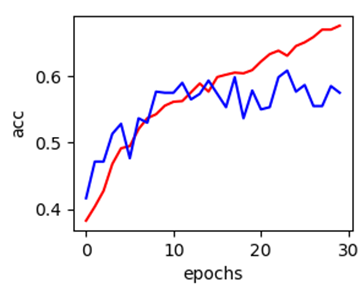
\includegraphics[width=\linewidth]{pre-processing-performance.png}
  \end{subfigure}
  \caption{Performance of Pre-Processing Changes}
  \label{fig:pre-processing-performance}
\end{figure}

From 30 epochs, the accuracy of the model reached close to 60\% which is an improvement to our model. Therefore these changes should be kept within our model. 
